% Original assessment and worked key governed by the supplied assessment brief.
% Build from this directory; all dependencies remain in this academic-year tree.
\makeatletter
\def\input@path{{../../../preamble/}}
\makeatother
\input{preamble_exams.tex}
\linespread{0.98}
\setlength{\parskip}{2pt}
\renewcommand{\arraystretch}{1.0}
\setlength{\emergencystretch}{2em}
\pgfplotsset{keyaxis/.style={axis lines=left,scaled ticks=false,
 xlabel={$x$ (USD)},grid=major,grid style={gray!15},
 tick label style={font=\small},label style={font=\small},clip=false}}
\title{Global Economics Exam Solutions\\Grade 10 --- Term 2 --- C1 and C2}
\author{}
\date{}
\makeatletter
\renewcommand{\@maketitle}{\begin{center}{\Large\bfseries\@title\par}\end{center}}
\renewcommand\subsection{\@startsection{subsection}{2}{\z@}{-1.4ex plus -.3ex}{.7ex}{\normalfont\large\bfseries}}
\makeatother
\hypersetup{pdftitle={Grade 10 Term 2 C1 and C2 Exam Solutions},pdfauthor={Global Economics}}
\begin{document}
\maketitle
\small
\setcounter{tocdepth}{1}
\phantomsection
\label{toc}
\tableofcontents
\section*{Learning objective}
Model discrete monetary outcomes in economic and financial contexts; derive and verify probability mass functions (PMFs), and construct and interpret cumulative distribution functions (CDFs) with tables and graphs.
\section*{Criteria assessment}
This standalone key authors the original questions required by the governing assessment brief and reproduces each task before its worked solution. Questions 1--2 assess C1; Questions 3--6 assess C2. Show reasoning and exact probabilities. All contextual rules are stated in ordinary language.

\textbf{Independent passing thresholds: C1 requires at least 4 out of 6 points; C2 requires at least 4 out of 14 points. Points cannot transfer between criteria.} The overall available total is 20 points. An overall total alone does not establish a pass in both criteria. These are the passing thresholds for this assessment; no cumulative policy is specified.
\section*{Evaluated criteria}
\begin{description}
\item[C1] Characterises discrete random variables in economic and financial contexts by identifying their support, probability mass function and possible outcomes.
\item[C2] Interprets PMFs and CDFs by verifying their defining properties and using them to calculate point, interval, cumulative, and complementary probabilities in financial contexts.
\end{description}


\begin{center}
\begin{tabular}{|c|c|c|}
	\hline\textbf{\textnumero} & \textbf{C1} & \textbf{C2} \\ \hline
	\ref*{sec:q1} & 3 & --- \\\hline
	\ref*{sec:q2} & 3 & --- \\\hline
	\ref*{sec:q3} & --- & 2 \\\hline
	\ref*{sec:q4} & --- & 2 \\\hline
	\ref*{sec:q5} & --- & 4 \\\hline
	\ref*{sec:q6} & --- & 6 \\\hline
	\textbf{Total} & \textbf{6} & \textbf{14} \\\hline
\end{tabular}
\end{center}


\textbf{Marking policy.} Question and criterion totals are fixed by the brief. Every task-level split and partial-credit breakdown below is proposed. Award stated fractions for demonstrated components, including valid alternative methods. Allow consistent follow-through after one arithmetic error when subsequent reasoning is correct; do not award a missing normalization or independent verification merely because a table looks plausible. Cap each task, question and criterion at its allocation.

\clearpage
\sectionScored{Online order contribution}{C1-\sml{3}}{sec:q1}

A small seller handles three orders, in first, second and third order. Each order independently has exactly two mutually exclusive possible outcomes: the buyer keeps it with probability 0.6, or cancels it with probability 0.4. These probabilities apply to every order. Each kept order contributes 5 USD and each cancellation contributes no money. A fixed handling cost of 4 USD is then deducted once from the combined contribution. There are no other receipts or costs. Record the net contribution for the three orders.

\textbf{Original Task 1 (proposed allocation).} \hyperref[sol:q1t1]{List every complete outcome in order and calculate its probability.} \score{1}


\subsection*{Worked solution to Task 1 \score{1}}
\label{sol:q1t1}

Write $K$ for kept and $C$ for cancelled. There are $2^3=8$ ordered complete outcomes. Independence permits multiplication within each triple; it does not make the triples equally likely.

\begin{center}
\begin{tabular}{ccc}\toprule
Ordered outcome & Product & Exact probability\\\midrule
$\mathrm{KKK}$ & $0.6\cdot0.6\cdot0.6$ & $27/125=0.216$\\
$\mathrm{KKC}$ & $0.6\cdot0.6\cdot0.4$ & $18/125=0.144$\\
$\mathrm{KCK}$ & $0.6\cdot0.4\cdot0.6$ & $18/125=0.144$\\
$\mathrm{KCC}$ & $0.6\cdot0.4\cdot0.4$ & $12/125=0.096$\\
$\mathrm{CKK}$ & $0.4\cdot0.6\cdot0.6$ & $18/125=0.144$\\
$\mathrm{CKC}$ & $0.4\cdot0.6\cdot0.4$ & $12/125=0.096$\\
$\mathrm{CCK}$ & $0.4\cdot0.4\cdot0.6$ & $12/125=0.096$\\
$\mathrm{CCC}$ & $0.4\cdot0.4\cdot0.4$ & $8/125=0.064$\\
\bottomrule\end{tabular}
\end{center}


The eight probabilities sum to $(3/5+2/5)^3=1$.

\textbf{Proposed partial credit.} 0.5 for all eight ordered outcomes; 0.5 for their probabilities using independent products. Total: 1 point.

\par\vspace{3mm}\secInicio[][sec:q1]

\textbf{Original Task 2 (proposed allocation).} \hyperref[sol:q1t2]{Define the random variable and its units. Map every complete outcome to a value, identify the support, and construct and verify the grouped PMF.} \score{1}


\subsection*{Worked solution to Task 2 \score{1}}
\label{sol:q1t2}

Let $X$ be the net contribution from the three orders, in USD. If $N$ is the number kept, $X=5N-4$. The table maps all eight outcomes and groups those with the same net contribution.

\begin{center}
\begin{tabular}{ccc}\toprule
$x$ (USD) & Complete outcomes & Grouped probability\\\midrule
$-4$ & $\mathrm{CCC}$ & $8/125=8/125$\\
$1$ & $\mathrm{KCC},\mathrm{CKC},\mathrm{CCK}$ & $12/125+12/125+12/125=36/125$\\
$6$ & $\mathrm{KKC},\mathrm{KCK},\mathrm{CKK}$ & $18/125+18/125+18/125=54/125$\\
$11$ & $\mathrm{KKK}$ & $27/125=27/125$\\
\bottomrule\end{tabular}
\end{center}


Thus $S_X=\{-4,1,6,11\}$ USD. The PMF is the last column, and is zero elsewhere. All masses are positive, and $(8+36+54+27)/125=1$. A negative value means the handling cost exceeds receipts.

\textbf{Proposed partial credit.} 0.125 for the variable and units; 0.25 for all outcome mappings; 0.125 for support; 0.375 for grouped PMF masses; 0.125 for positivity and normalization checks. Total: 1 point.

\par\vspace{3mm}\secInicio[][sec:q1]

\textbf{Original Task 3 (proposed allocation).} \hyperref[sol:q1t3]{Calculate and interpret the probability that the net contribution is at least 6 USD.} \score{1}


\subsection*{Worked solution to Task 3 \score{1}}
\label{sol:q1t3}

From the grouped PMF, $P(X\geq6)=p_X(6)+p_X(11)=54/125+27/125=81/125=0.648$. The seller earns a net contribution of at least 6 USD with probability 64.8\%; this happens exactly when at least two orders are kept.

\textbf{Proposed partial credit.} 0.5 for selecting and adding the correct masses; 0.5 for the contextual interpretation. Total: 1 point. Question total: 3 points for C1.

\par\vspace{3mm}\secInicio[][sec:q1]

\clearpage
\sectionScored{Two supplier loyalty credits}{C1-\sml{3}}{sec:q2}

A retailer receives one loyalty credit from each of two suppliers. The suppliers award credits independently. Each has exactly three mutually exclusive possible outcomes: no credit, a 3 USD credit, or an 8 USD credit. For the first supplier these probabilities are 0.2, 0.5 and 0.3, respectively. For the second supplier they are 0.4, 0.4 and 0.2, respectively. Add both credits; there are no other adjustments. Record the total credit, keeping first-supplier then second-supplier order.

\textbf{Original Task 1 (proposed allocation).} \hyperref[sol:q2t1]{List every complete ordered outcome and calculate its probability.} \score{1}


\subsection*{Worked solution to Task 1 \score{1}}
\label{sol:q2t1}

Each supplier has three possible outcomes, giving $3^2=9$ ordered pairs. Write a pair as its two credit amounts, in USD. Multiply the appropriate probabilities by independence.

\begin{center}
\begin{tabular}{ccc}\toprule
Ordered credit outcome (USD) & Product & Exact probability\\\midrule
$(0,0)$ & $0.2\cdot0.4$ & $2/25=0.08$\\
$(0,3)$ & $0.2\cdot0.4$ & $2/25=0.08$\\
$(0,8)$ & $0.2\cdot0.2$ & $1/25=0.04$\\
$(3,0)$ & $0.5\cdot0.4$ & $1/5=0.20$\\
$(3,3)$ & $0.5\cdot0.4$ & $1/5=0.20$\\
$(3,8)$ & $0.5\cdot0.2$ & $1/10=0.10$\\
$(8,0)$ & $0.3\cdot0.4$ & $3/25=0.12$\\
$(8,3)$ & $0.3\cdot0.4$ & $3/25=0.12$\\
$(8,8)$ & $0.3\cdot0.2$ & $3/50=0.06$\\
\bottomrule\end{tabular}
\end{center}


Exhaustiveness check: $(0.2+0.5+0.3)(0.4+0.4+0.2)=1$.

\textbf{Proposed partial credit.} 0.5 for all nine ordered pairs; 0.5 for independent product probabilities. Total: 1 point.

\par\vspace{3mm}\secInicio[][sec:q2]

\textbf{Original Task 2 (proposed allocation).} \hyperref[sol:q2t2]{Define the random variable and units; map every outcome to a value; identify the support; construct and verify the grouped PMF.} \score{1}


\subsection*{Worked solution to Task 2 \score{1}}
\label{sol:q2t2}

Let $X$ be the total loyalty credit from the two suppliers, in USD. Add the two amounts in each pair. The complete mapping and grouped PMF are:

\begin{center}
\begin{tabular}{ccc}\toprule
$x$ (USD) & Ordered outcomes & Grouped probability\\\midrule
$0$ & $(0,0)$ & $2/25=2/25$\\
$3$ & $(0,3),(3,0)$ & $2/25+1/5=7/25$\\
$6$ & $(3,3)$ & $1/5=1/5$\\
$8$ & $(0,8),(8,0)$ & $1/25+3/25=4/25$\\
$11$ & $(3,8),(8,3)$ & $1/10+3/25=11/50$\\
$16$ & $(8,8)$ & $3/50=3/50$\\
\bottomrule\end{tabular}
\end{center}


The support is $S_X=\{0,3,6,8,11,16\}$ USD, with zero mass elsewhere. All masses are positive and $(4+14+10+8+11+3)/50=50/50=1$. Reversing a pair can preserve its monetary value while changing its probability.

\textbf{Proposed partial credit.} 0.125 for variable and units; 0.25 for all mappings; 0.125 for support; 0.375 for grouped masses; 0.125 for positivity and normalization checks. Total: 1 point.

\par\vspace{3mm}\secInicio[][sec:q2]

\textbf{Original Task 3 (proposed allocation).} \hyperref[sol:q2t3]{Calculate and interpret the probability that the total credit is at least 11 USD.} \score{1}


\subsection*{Worked solution to Task 3 \score{1}}
\label{sol:q2t3}

$P(X\geq11)=p_X(11)+p_X(16)=11/50+3/50=7/25=0.28$. The retailer receives a total credit of at least 11 USD with probability 28\%; the qualifying pairs are $(3,8),(8,3),(8,8)$.

\textbf{Proposed partial credit.} 0.5 for selecting and adding the correct masses; 0.5 for the contextual interpretation. Total: 1 point. Question total: 3 points for C1. Criterion C1 total: 6 points; independent pass: at least 4 points.

\par\vspace{3mm}\secInicio[][sec:q2]

\clearpage
\sectionScored{Local parcel delivery fees}{C2-\sml{2}}{sec:q3}

\textbf{Basic Type A.} A cooperative sends one parcel using exactly one of eight exhaustive, mutually exclusive delivery methods: walking courier, bicycle, cargo bicycle, motorcycle, car, van, refrigerated van or truck. Their probabilities are 0.10, 0.10, 0.15, 0.20, 0.15, 0.10, 0.10 and 0.10, respectively. The corresponding fixed handling fees are 0, 0, 2, 4, 7, 11, 16 and 23 USD, respectively. No other handling charges apply. Record the handling fee for the parcel.

\textbf{Original Task 1 (proposed allocation).} \hyperref[sol:q3t1]{Define the random variable and support; derive and verify the grouped PMF; produce its table and a labeled graph with actual monetary spacing.} \score{1}


\subsection*{Worked solution to Task 1 \score{1}}
\label{sol:q3t1}

Let $X$ be the handling fee for one parcel, in USD. Map the supplied categories to payments:

\begin{center}
\begin{tabular}{ccc}\toprule
Category & Given probability & $X$ (USD)\\\midrule
Walking courier & $0.10=2/20$ & $0$\\
Bicycle & $0.10=2/20$ & $0$\\
Cargo bicycle & $0.15=3/20$ & $2$\\
Motorcycle & $0.20=4/20$ & $4$\\
Car & $0.15=3/20$ & $7$\\
Van & $0.10=2/20$ & $11$\\
Refrigerated van & $0.10=2/20$ & $16$\\
Truck & $0.10=2/20$ & $23$\\
\bottomrule\end{tabular}
\end{center}


The walking courier and bicycle are distinct outcomes sharing a zero fee, so $p_X(0)=0.10+0.10=0.20=4/20$. Every other method has its own fee and retains its supplied probability.

$S_X=\{0,2,4,7,11,16,23\}$ USD. There are eight elementary outcomes but seven distinct monetary values. Add probabilities of mutually exclusive categories sharing a value, because the events cannot occur together.

\begin{center}
\begin{tabular}{cc}\toprule
$x$ (USD) & $p_X(x)$\\\midrule
$0$ & $4/20$\\
$2$ & $3/20$\\
$4$ & $4/20$\\
$7$ & $3/20$\\
$11$ & $2/20$\\
$16$ & $2/20$\\
$23$ & $2/20$\\
\bottomrule\end{tabular}
\end{center}


\begin{center}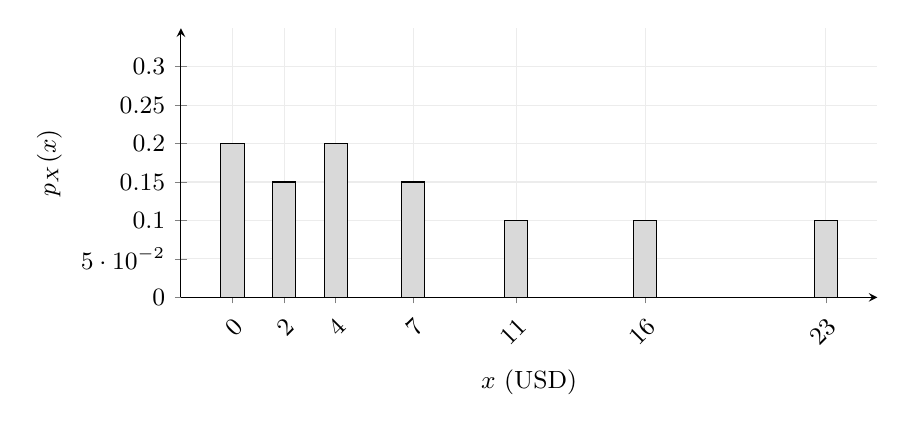
\begin{tikzpicture}
\begin{axis}[keyaxis,width=.86\linewidth,height=5cm,xmin=-2,xmax=25,ymin=0,ymax=.35,xtick={0,2,4,7,11,16,23},xticklabel style={rotate=45,anchor=north east},ylabel={$p_X(x)$},ytick={0,.05,.1,.15,.2,.25,.3}]
\draw[fill=black!15] (axis cs:-0.45,0) rectangle (axis cs:0.45,4/20);
\draw[fill=black!15] (axis cs:1.55,0) rectangle (axis cs:2.45,3/20);
\draw[fill=black!15] (axis cs:3.55,0) rectangle (axis cs:4.45,4/20);
\draw[fill=black!15] (axis cs:6.55,0) rectangle (axis cs:7.45,3/20);
\draw[fill=black!15] (axis cs:10.55,0) rectangle (axis cs:11.45,2/20);
\draw[fill=black!15] (axis cs:15.55,0) rectangle (axis cs:16.45,2/20);
\draw[fill=black!15] (axis cs:22.55,0) rectangle (axis cs:23.45,2/20);
\end{axis}\end{tikzpicture}\end{center}

\textbf{PMF check.} Every listed mass is strictly positive, and $4+3+4+3+2+2+2=20$, so the masses sum to $20/20=1$. Set $p_X(x)=0$ outside the support. The graph places bars at the actual monetary values; gaps carry no mass.

\textbf{Proposed partial credit.} 0.25 for variable, units and support; 0.25 for category mapping, grouping and the PMF table; 0.25 for the labeled, correctly spaced graph; 0.25 for positivity and normalization. Total: 1 point.

\par\vspace{3mm}\secInicio[][sec:q3]

\clearpage
\textbf{Question 3 --- continued}

\textbf{Original Task 2 (proposed allocation).} \hyperref[sol:q3t2]{Construct the complete CDF table, including both tails, and draw a labeled step graph. Use open and filled endpoints correctly and preserve actual monetary spacing. Verify the defining CDF properties and that its jumps equal the PMF masses.} \score{1}


\subsection*{Worked solution to Task 2 \score{1}}
\label{sol:q3t2}

For $F_X(x)=P(X\leq x)$, add masses in increasing fee order. The successive cumulative numerators are $4,7,11,14,16,18,20$, all over $20$.

\begin{center}
\begin{tabular}{cc}\toprule
Cutoff interval (USD) & $F_X(x)$\\\midrule
$x<0$ & $0$\\
$0\leq x<2$ & $4/20$\\
$2\leq x<4$ & $7/20$\\
$4\leq x<7$ & $11/20$\\
$7\leq x<11$ & $14/20$\\
$11\leq x<16$ & $16/20$\\
$16\leq x<23$ & $18/20$\\
$x\geq 23$ & $1$\\
\bottomrule\end{tabular}
\end{center}


\begin{center}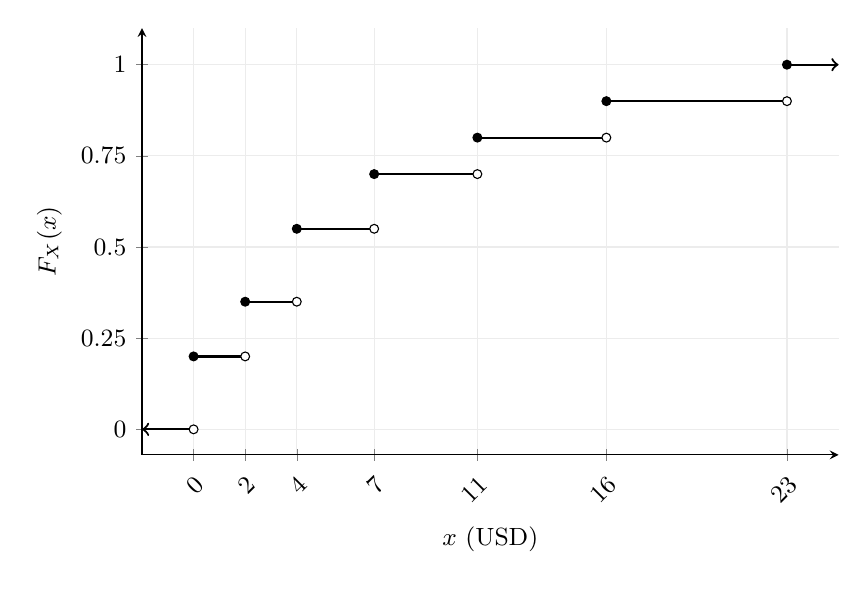
\begin{tikzpicture}
\begin{axis}[keyaxis,width=.86\linewidth,height=7cm,xmin=-2,xmax=25,ymin=-.07,ymax=1.1,xtick={0,2,4,7,11,16,23},xticklabel style={rotate=45,anchor=north east},ytick={0,.25,.5,.75,1},ylabel={$F_X(x)$}]
\addplot[thick,<-] coordinates {(-2,0)(0,0)};
\addplot[thick] coordinates {(0,4/20)(2,4/20)};
\addplot[thick] coordinates {(2,7/20)(4,7/20)};
\addplot[thick] coordinates {(4,11/20)(7,11/20)};
\addplot[thick] coordinates {(7,14/20)(11,14/20)};
\addplot[thick] coordinates {(11,16/20)(16,16/20)};
\addplot[thick] coordinates {(16,18/20)(23,18/20)};
\addplot[thick,->] coordinates {(23,1)(25,1)};
\addplot[only marks,mark=*,mark size=1.6pt,mark options={fill=white}] coordinates {(0,0/20)(2,4/20)(4,7/20)(7,11/20)(11,14/20)(16,16/20)(23,18/20)};
\addplot[only marks,mark=*,mark size=1.6pt] coordinates {(0,4/20)(2,7/20)(4,11/20)(7,14/20)(11,16/20)(16,18/20)(23,20/20)};
\end{axis}\end{tikzpicture}\end{center}

\textbf{CDF checks.} The table covers every real cutoff. Heights lie in $[0,1]$ and never decrease. Each horizontal segment includes its left endpoint and excludes its right endpoint: the filled point gives the value at a jump, so the CDF is right-continuous. Arrows extend the tails to $-\infty$ and $+\infty$, where the limits are 0 and 1.

In support order, subtracting successive cumulative numerators (starting at zero) gives $4,3,4,3,2,2,2$. Hence each jump is its PMF mass over $20$: $F_X(a)-F_X(a^-)=p_X(a)$. At unsupported cutoffs both the jump and the mass are zero.

\textbf{Proposed partial credit.} 0.25 for cumulative sums; 0.25 for the complete interval table and tails; 0.25 for the labeled, correctly spaced step graph and endpoints; 0.25 for the CDF and jump checks. Total: 1 point.

\par\vspace{3mm}\secInicio[][sec:q3]

\textbf{Question total: 2 points for C2.}

\clearpage
\sectionScored{Warranty service payouts}{C2-\sml{2}}{sec:q4}

\textbf{Basic Type A.} A warranty provider classifies one claim in exactly one of eight exhaustive, mutually exclusive categories: no service, remote diagnosis, software reset, minor repair, major repair, replacement, store credit or cash refund. These eight named categories are the distinct outcomes in the sample space. Their probabilities are 0.20, 0.10, 0.15, 0.15, 0.10, 0.15, 0.05 and 0.10, respectively; do not assume equal likelihood. The corresponding payouts are 0, 2, 4, 6, 10, 15, 15 and 25 USD, respectively. Count store credit at its face value as a payout. Each payout is fixed for its category, and no additional payments apply. Record the provider's payout for one claim.

\textbf{Original Task 1 (proposed allocation).} \hyperref[sol:q4t1]{Define the random variable and support; derive and verify the grouped PMF; produce its table and a labeled graph with actual monetary spacing.} \score{1}


\subsection*{Worked solution to Task 1 \score{1}}
\label{sol:q4t1}

Let $X$ be the provider payout for one claim, in USD. Map the supplied categories to payments:

\begin{center}
\begin{tabular}{ccc}\toprule
Category & Given probability & $X$ (USD)\\\midrule
No service & $0.20=4/20$ & $0$\\
Remote diagnosis & $0.10=2/20$ & $2$\\
Software reset & $0.15=3/20$ & $4$\\
Minor repair & $0.15=3/20$ & $6$\\
Major repair & $0.10=2/20$ & $10$\\
Replacement & $0.15=3/20$ & $15$\\
Store credit & $0.05=1/20$ & $15$\\
Cash refund & $0.10=2/20$ & $25$\\
\bottomrule\end{tabular}
\end{center}


Replacement and store credit are distinct outcomes sharing a 15 USD payout, so $p_X(15)=0.15+0.05=0.20=4/20$. Store credit counts at face value. Every other category has its own payout and retains its supplied probability.

$S_X=\{0,2,4,6,10,15,25\}$ USD. There are eight elementary outcomes but seven distinct monetary values. Add probabilities of mutually exclusive categories sharing a value, because the events cannot occur together.

\begin{center}
\begin{tabular}{cc}\toprule
$x$ (USD) & $p_X(x)$\\\midrule
$0$ & $4/20$\\
$2$ & $2/20$\\
$4$ & $3/20$\\
$6$ & $3/20$\\
$10$ & $2/20$\\
$15$ & $4/20$\\
$25$ & $2/20$\\
\bottomrule\end{tabular}
\end{center}


\begin{center}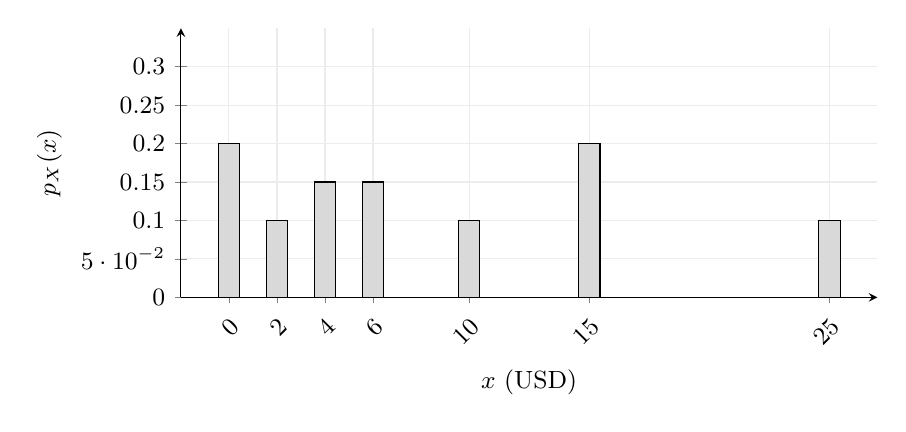
\begin{tikzpicture}
\begin{axis}[keyaxis,width=.86\linewidth,height=5cm,xmin=-2,xmax=27,ymin=0,ymax=.35,xtick={0,2,4,6,10,15,25},xticklabel style={rotate=45,anchor=north east},ylabel={$p_X(x)$},ytick={0,.05,.1,.15,.2,.25,.3}]
\draw[fill=black!15] (axis cs:-0.45,0) rectangle (axis cs:0.45,4/20);
\draw[fill=black!15] (axis cs:1.55,0) rectangle (axis cs:2.45,2/20);
\draw[fill=black!15] (axis cs:3.55,0) rectangle (axis cs:4.45,3/20);
\draw[fill=black!15] (axis cs:5.55,0) rectangle (axis cs:6.45,3/20);
\draw[fill=black!15] (axis cs:9.55,0) rectangle (axis cs:10.45,2/20);
\draw[fill=black!15] (axis cs:14.55,0) rectangle (axis cs:15.45,4/20);
\draw[fill=black!15] (axis cs:24.55,0) rectangle (axis cs:25.45,2/20);
\end{axis}\end{tikzpicture}\end{center}

\textbf{PMF check.} Every listed mass is strictly positive, and $4+2+3+3+2+4+2=20$, so the masses sum to $20/20=1$. Set $p_X(x)=0$ outside the support. The graph places bars at the actual monetary values; gaps carry no mass.

\textbf{Proposed partial credit.} 0.25 for variable, units and support; 0.25 for category mapping, grouping and the PMF table; 0.25 for the labeled, correctly spaced graph; 0.25 for positivity and normalization. Total: 1 point.

\par\vspace{3mm}\secInicio[][sec:q4]

\clearpage
\textbf{Question 4 --- continued}

\textbf{Original Task 2 (proposed allocation).} \hyperref[sol:q4t2]{Construct the complete CDF table, including both tails, and draw a labeled step graph. Use open and filled endpoints correctly and preserve actual monetary spacing. Verify the defining CDF properties and that its jumps equal the PMF masses.} \score{1}


\subsection*{Worked solution to Task 2 \score{1}}
\label{sol:q4t2}

For $F_X(x)=P(X\leq x)$, add masses in increasing payout order. The successive cumulative numerators are $4,6,9,12,14,18,20$, all over $20$.

\begin{center}
\begin{tabular}{cc}\toprule
Cutoff interval (USD) & $F_X(x)$\\\midrule
$x<0$ & $0$\\
$0\leq x<2$ & $4/20$\\
$2\leq x<4$ & $6/20$\\
$4\leq x<6$ & $9/20$\\
$6\leq x<10$ & $12/20$\\
$10\leq x<15$ & $14/20$\\
$15\leq x<25$ & $18/20$\\
$x\geq 25$ & $1$\\
\bottomrule\end{tabular}
\end{center}


\begin{center}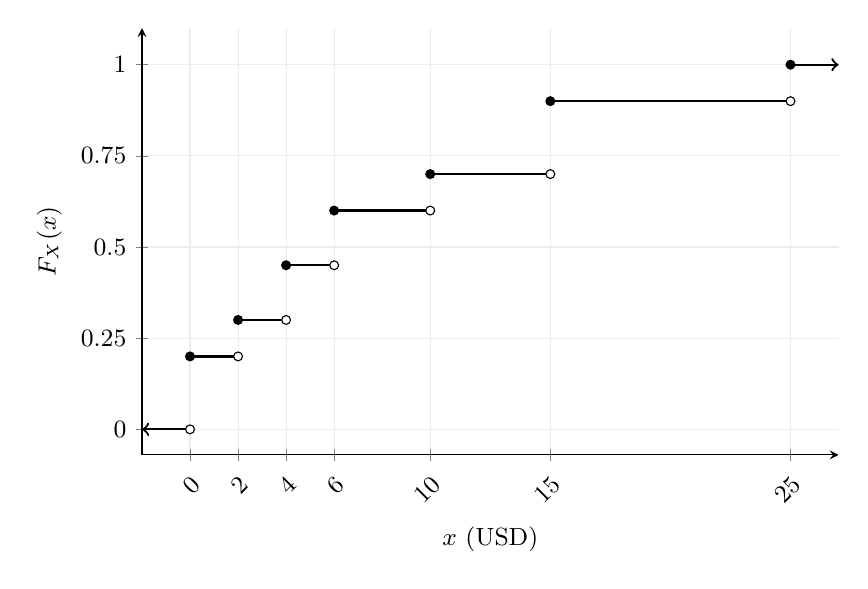
\begin{tikzpicture}
\begin{axis}[keyaxis,width=.86\linewidth,height=7cm,xmin=-2,xmax=27,ymin=-.07,ymax=1.1,xtick={0,2,4,6,10,15,25},xticklabel style={rotate=45,anchor=north east},ytick={0,.25,.5,.75,1},ylabel={$F_X(x)$}]
\addplot[thick,<-] coordinates {(-2,0)(0,0)};
\addplot[thick] coordinates {(0,4/20)(2,4/20)};
\addplot[thick] coordinates {(2,6/20)(4,6/20)};
\addplot[thick] coordinates {(4,9/20)(6,9/20)};
\addplot[thick] coordinates {(6,12/20)(10,12/20)};
\addplot[thick] coordinates {(10,14/20)(15,14/20)};
\addplot[thick] coordinates {(15,18/20)(25,18/20)};
\addplot[thick,->] coordinates {(25,1)(27,1)};
\addplot[only marks,mark=*,mark size=1.6pt,mark options={fill=white}] coordinates {(0,0/20)(2,4/20)(4,6/20)(6,9/20)(10,12/20)(15,14/20)(25,18/20)};
\addplot[only marks,mark=*,mark size=1.6pt] coordinates {(0,4/20)(2,6/20)(4,9/20)(6,12/20)(10,14/20)(15,18/20)(25,20/20)};
\end{axis}\end{tikzpicture}\end{center}

\textbf{CDF checks.} The table covers every real cutoff. Heights lie in $[0,1]$ and never decrease. Each horizontal segment includes its left endpoint and excludes its right endpoint: the filled point gives the value at a jump, so the CDF is right-continuous. Arrows extend the tails to $-\infty$ and $+\infty$, where the limits are 0 and 1.

In support order, subtracting successive cumulative numerators (starting at zero) gives $4,2,3,3,2,4,2$. Hence each jump is its PMF mass over $20$: $F_X(a)-F_X(a^-)=p_X(a)$. At unsupported cutoffs both the jump and the mass are zero.

\textbf{Proposed partial credit.} 0.25 for cumulative sums; 0.25 for the complete interval table and tails; 0.25 for the labeled, correctly spaced step graph and endpoints; 0.25 for the CDF and jump checks. Total: 1 point.

\par\vspace{3mm}\secInicio[][sec:q4]

\textbf{Question total: 2 points for C2.}

\clearpage
\sectionScored{Marketplace account credits}{C2-\sml{4}}{sec:q5}

\textbf{Advanced Type A.} For one purchase, a marketplace awards exactly one account credit: 0, 2, 5, 9, 14 or 20 USD. These are all possible credits and their categories are mutually exclusive. A 2 USD credit is twice as likely as no credit. A 5 USD credit is as likely as no credit and a 2 USD credit combined. A 9 USD credit is twice as likely as a 5 USD credit. A 14 USD credit is half as likely as a 9 USD credit. A 20 USD credit is as likely as the 2 USD and 14 USD credits combined. There are no other payments or adjustments. Determine the probabilities from these likelihood relationships and record the account credit.

\textbf{Original Task 1 (proposed allocation).} \hyperref[sol:q5t1]{Define the random variable and support. Derive the six probabilities using normalization, verify the PMF, and produce its table and labeled graph.} \score{2}


\subsection*{Worked solution to Task 1 \score{2}}
\label{sol:q5t1}

Let $X$ be the account credit for one purchase, in USD, with $S_X=\{0,2,5,9,14,20\}$. Set $a=P(X=0)$. Since the categories are mutually exclusive, a combined likelihood is a sum. Translate the relationships in their stated order:
\begin{align*}
p_X(0)&=a,&p_X(2)&=2a,\\
p_X(5)&=a+2a=3a,&p_X(9)&=2(3a)=6a,\\
p_X(14)&=\tfrac12(6a)=3a,&p_X(20)&=2a+3a=5a.
\end{align*}
Normalization gives
\[
a+2a+3a+6a+3a+5a=1,\qquad 20a=1,\qquad a=\frac1{20}.
\]
Every probability is now uniquely determined: all depend on the single baseline, whose positive coefficient in the normalization equation is 20. No probability is zero. Each credit is already a distinct monetary value, so no additional grouping is needed.

\begin{center}
\begin{tabular}{cc}\toprule
$x$ (USD) & $p_X(x)$\\\midrule
$0$ & $1/20$\\
$2$ & $2/20=1/10$\\
$5$ & $3/20$\\
$9$ & $6/20=3/10$\\
$14$ & $3/20$\\
$20$ & $5/20=1/4$\\
\bottomrule\end{tabular}
\end{center}


\begin{center}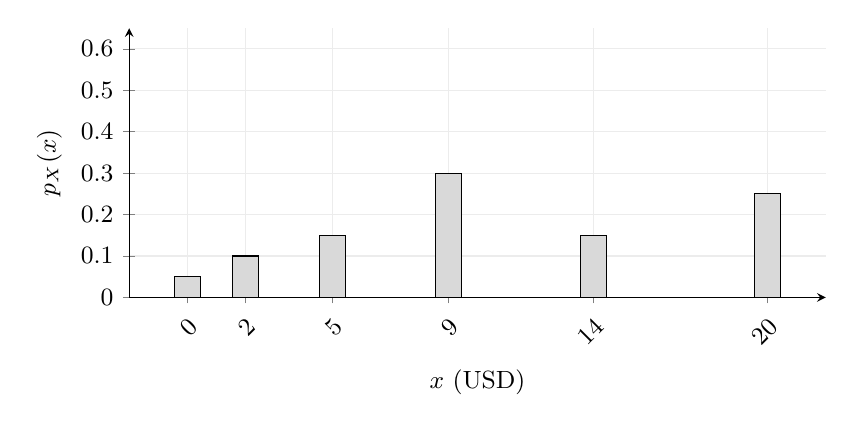
\begin{tikzpicture}
\begin{axis}[keyaxis,width=.86\linewidth,height=5cm,xmin=-2,xmax=22,ymin=0,ymax=.65,xtick={0,2,5,9,14,20},xticklabel style={rotate=45,anchor=north east},ylabel={$p_X(x)$},ytick={0,.1,.2,.3,.4,.5,.6}]

\draw[fill=black!15] (axis cs:-0.45,0) rectangle (axis cs:0.45,1/20);

\draw[fill=black!15] (axis cs:1.55,0) rectangle (axis cs:2.45,2/20);

\draw[fill=black!15] (axis cs:4.55,0) rectangle (axis cs:5.45,3/20);

\draw[fill=black!15] (axis cs:8.55,0) rectangle (axis cs:9.45,6/20);

\draw[fill=black!15] (axis cs:13.55,0) rectangle (axis cs:14.45,3/20);

\draw[fill=black!15] (axis cs:19.55,0) rectangle (axis cs:20.45,5/20);

\end{axis}\end{tikzpicture}\end{center}

\textbf{PMF check.} Every listed mass is strictly positive, and $1+2+3+6+3+5=20$, so the masses sum to $20/20=1$. Set $p_X(x)=0$ outside the support. The graph places bars at the actual monetary values; gaps carry no mass.

\textbf{Relationship check.} The numerators satisfy $2=2(1)$, $3=1+2$, $6=2(3)$, $3=6/2$, and $5=2+3$, exactly reproducing all five verbal relationships.

\textbf{Proposed partial credit.} 0.25 for variable, units and support; 0.75 for translating the relationships and solving normalization; 0.5 for all six PMF entries; 0.25 for the labeled, correctly spaced graph; 0.25 for positivity, normalization and relationship checks. Total: 2 points.

\par\vspace{3mm}\secInicio[][sec:q5]

\clearpage
\textbf{Question 5 --- continued}

\textbf{Original Task 2 (proposed allocation).} \hyperref[sol:q5t2]{Construct the complete CDF table, including both tails, and draw a labeled step graph. Use open and filled endpoints correctly and preserve actual monetary spacing. Verify the defining CDF properties and that its jumps equal the PMF masses.} \score{2}


\subsection*{Worked solution to Task 2 \score{2}}
\label{sol:q5t2}

For $F_X(x)=P(X\leq x)$, add masses in increasing payout order. The successive cumulative numerators are $1,3,6,12,15,20$, all over $20$.

\begin{center}
\begin{tabular}{cc}\toprule
Cutoff interval (USD) & $F_X(x)$\\\midrule
$x<0$ & $0$\\
$0\leq x<2$ & $1/20$\\
$2\leq x<5$ & $3/20$\\
$5\leq x<9$ & $3/10$\\
$9\leq x<14$ & $3/5$\\
$14\leq x<20$ & $3/4$\\
$x\geq 20$ & $1$\\
\bottomrule\end{tabular}
\end{center}


\begin{center}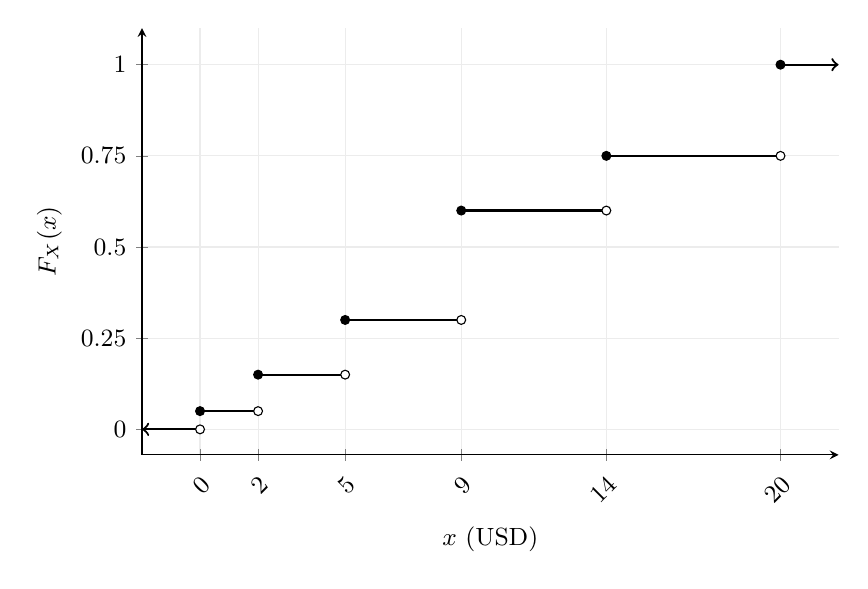
\begin{tikzpicture}
\begin{axis}[keyaxis,width=.86\linewidth,height=7cm,xmin=-2,xmax=22,ymin=-.07,ymax=1.1,xtick={0,2,5,9,14,20},xticklabel style={rotate=45,anchor=north east},ytick={0,.25,.5,.75,1},ylabel={$F_X(x)$}]

\addplot[thick,<-] coordinates {(-2,0)(0,0)};

\addplot[thick] coordinates {(0,1/20)(2,1/20)};

\addplot[thick] coordinates {(2,3/20)(5,3/20)};

\addplot[thick] coordinates {(5,6/20)(9,6/20)};

\addplot[thick] coordinates {(9,12/20)(14,12/20)};

\addplot[thick] coordinates {(14,15/20)(20,15/20)};

\addplot[thick,->] coordinates {(20,1)(22,1)};

\addplot[only marks,mark=*,mark size=1.6pt,mark options={fill=white}] coordinates {(0,0/20)(2,1/20)(5,3/20)(9,6/20)(14,12/20)(20,15/20)};

\addplot[only marks,mark=*,mark size=1.6pt] coordinates {(0,1/20)(2,3/20)(5,6/20)(9,12/20)(14,15/20)(20,20/20)};

\end{axis}\end{tikzpicture}\end{center}

\textbf{CDF checks.} The table covers every real cutoff. Heights lie in $[0,1]$ and never decrease. Each horizontal segment includes its left endpoint and excludes its right endpoint: the filled point gives the value at a jump, so the CDF is right-continuous. Arrows extend the tails to $-\infty$ and $+\infty$, where the limits are 0 and 1.

In support order, subtracting successive cumulative numerators (starting at zero) gives $1,2,3,6,3,5$. Hence each jump is its PMF mass over $20$: $F_X(a)-F_X(a^-)=p_X(a)$. At unsupported cutoffs both the jump and the mass are zero.

\textbf{Proposed partial credit.} 0.5 for cumulative sums; 0.5 for the complete interval table and tails; 0.5 for the labeled, correctly spaced step graph and endpoints; 0.5 for the CDF and jump checks. Total: 2 points.

\par\vspace{3mm}\secInicio[][sec:q5]

\textbf{Question total: 4 points for C2.}

\clearpage
\sectionScored{Community market prize tickets}{C2-\sml{6}}{sec:q6}

\textbf{Advanced Type B.} A community market has nine physically distinct prize tickets: four worth 0 USD each, three worth 5 USD each and two worth 12 USD each. Choose a subset of three tickets uniformly without replacement, so every subset of three physically distinct tickets has the same chance. Ignore selection order. First add the face values. Then add one bonus of 7 USD if the selected subset contains at least one 5 USD ticket and at least one 12 USD ticket; otherwise add no bonus. Finally, if this adjusted amount exceeds 25 USD, pay only 25 USD; otherwise pay the adjusted amount. No other payments or deductions apply. Record the final payout.

\textbf{Original Task 1 (proposed allocation).} \hyperref[sol:q6t1]{Define the random variable and support. Count the distinct-ticket selections, apply the bonus and then the cap, aggregate equal final payouts, and derive and verify the PMF. Produce its table and labeled graph.} \score{3}


\subsection*{Worked solution to Task 1 \score{3}}
\label{sol:q6t1}

Let $X$ be the final payout for one three-ticket subset, in USD. Label the physical tickets $Z_1,\ldots,Z_4$, $L_1,\ldots,L_3$, and $H_1,H_2$, with values 0, 5 and 12 USD. There are
\[
\binom93=\frac{9\cdot8\cdot7}{3\cdot2\cdot1}=84
\]
equally likely unordered subsets, each with probability $1/84$. A composition records $(a,b,c)$, the counts of zero-, five- and twelve-dollar tickets. Feasible counts satisfy $a+b+c=3$, $0\leq a\leq4$, $0\leq b\leq3$, and $0\leq c\leq2$. The number of subsets with that composition is
\[
N(a,b,c)=\binom4a\binom3b\binom2c,\qquad P(a,b,c)=\frac{N(a,b,c)}{84}.
\]
Define $I=1$ if $b\geq1$ and $c\geq1$, and $I=0$ otherwise. The face sum is $5b+12c$; the adjusted amount is $Y=5b+12c+7I$; finally $X=\min\{Y,25\}$. The bonus is added once, before the cap.

\begingroup\renewcommand{\arraystretch}{1.35}

\begin{center}
\begin{tabular}{ccccccc}\toprule
$(a,b,c)$ & Subset count & Probability & Face sum & Bonus & $Y$ & $X$\\\midrule
$(3,0,0)$ & $\binom4{3}\binom3{0}\binom2{0}=4$ & $4/84$ & 0 & 0 & 0 & 0\\
$(2,1,0)$ & $\binom4{2}\binom3{1}\binom2{0}=18$ & $18/84$ & 5 & 0 & 5 & 5\\
$(1,2,0)$ & $\binom4{1}\binom3{2}\binom2{0}=12$ & $12/84$ & 10 & 0 & 10 & 10\\
$(0,3,0)$ & $\binom4{0}\binom3{3}\binom2{0}=1$ & $1/84$ & 15 & 0 & 15 & 15\\
$(2,0,1)$ & $\binom4{2}\binom3{0}\binom2{1}=12$ & $12/84$ & 12 & 0 & 12 & 12\\
$(1,1,1)$ & $\binom4{1}\binom3{1}\binom2{1}=24$ & $24/84$ & 17 & 7 & 24 & 24\\
$(0,2,1)$ & $\binom4{0}\binom3{2}\binom2{1}=6$ & $6/84$ & 22 & 7 & 29 & 25\\
$(1,0,2)$ & $\binom4{1}\binom3{0}\binom2{2}=4$ & $4/84$ & 24 & 0 & 24 & 24\\
$(0,1,2)$ & $\binom4{0}\binom3{1}\binom2{2}=3$ & $3/84$ & 29 & 7 & 36 & 25\\
\bottomrule\end{tabular}
\end{center}


\endgroup

All monetary columns are in USD. These nine compositions are exhaustive: list $c=0,1,2$ and every feasible $b$, then $a=3-b-c$. Their counts sum to $4+18+12+1+12+24+6+4+3=84$. Compositions are not equally likely: for example, $(1,1,1)$ represents 24 subsets, whereas $(0,3,0)$ represents only one.

\textbf{Aggregation.} The 24 USD payout comes from $(1,1,1)$ (24 subsets after the bonus) and $(1,0,2)$ (4 subsets without a bonus), so $p_X(24)=(24+4)/84=28/84$. The cap merges the adjusted amounts 29 and 36 USD from $(0,2,1)$ and $(0,1,2)$, so $p_X(25)=(6+3)/84=9/84$. Each other payout arises from one composition.

Thus $S_X=\{0,5,10,12,15,24,25\}$ USD. The cap binds only when the adjusted amount is greater than 25 USD; the 24 USD payout remains unchanged.

\par\vspace{3mm}\secInicio[][sec:q6]

\clearpage\textbf{Question 6 --- Task 1 continued: grouped PMF and graph}

\begin{center}
\begin{tabular}{cc}\toprule
$x$ (USD) & $p_X(x)$\\\midrule
$0$ & $4/84=1/21$\\
$5$ & $18/84=3/14$\\
$10$ & $12/84=1/7$\\
$12$ & $12/84=1/7$\\
$15$ & $1/84$\\
$24$ & $28/84=1/3$\\
$25$ & $9/84=3/28$\\
\bottomrule\end{tabular}
\end{center}


\begin{center}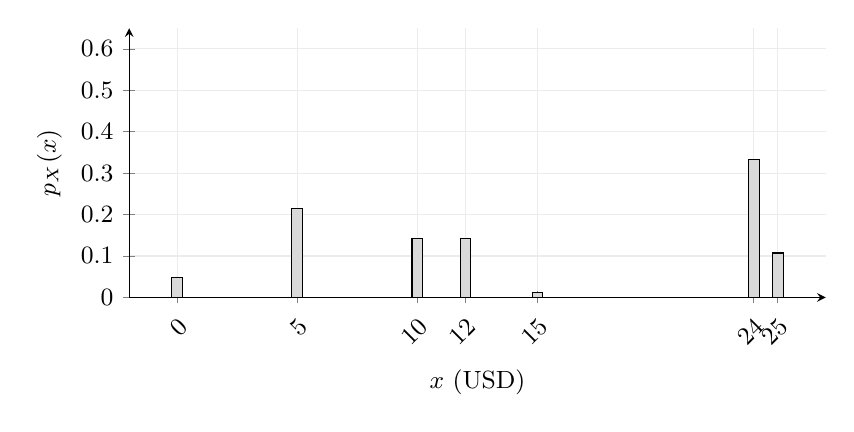
\begin{tikzpicture}
\begin{axis}[keyaxis,width=.86\linewidth,height=5cm,xmin=-2,xmax=27,ymin=0,ymax=.65,xtick={0,5,10,12,15,24,25},xticklabel style={rotate=45,anchor=north east},ylabel={$p_X(x)$},ytick={0,.1,.2,.3,.4,.5,.6}]

\draw[fill=black!15] (axis cs:-0.225,0) rectangle (axis cs:0.225,4/84);

\draw[fill=black!15] (axis cs:4.775,0) rectangle (axis cs:5.225,18/84);

\draw[fill=black!15] (axis cs:9.775,0) rectangle (axis cs:10.225,12/84);

\draw[fill=black!15] (axis cs:11.775,0) rectangle (axis cs:12.225,12/84);

\draw[fill=black!15] (axis cs:14.775,0) rectangle (axis cs:15.225,1/84);

\draw[fill=black!15] (axis cs:23.775,0) rectangle (axis cs:24.225,28/84);

\draw[fill=black!15] (axis cs:24.775,0) rectangle (axis cs:25.225,9/84);

\end{axis}\end{tikzpicture}\end{center}

\textbf{PMF check.} Every listed mass is strictly positive, and $4+18+12+12+1+28+9=84$, so the masses sum to $84/84=1$. Set $p_X(x)=0$ outside the support. The graph places bars at the actual monetary values; gaps carry no mass.

\textbf{Proposed partial credit.} 0.25 for variable, units and support; 0.75 for the denominator and exhaustive composition counts; 0.75 for the bonus, cap and aggregation; 0.5 for the grouped PMF table; 0.5 for the labeled, correctly spaced graph; 0.25 for positivity and normalization checks. Total: 3 points.

\par\vspace{3mm}\secInicio[][sec:q6]

\clearpage
\textbf{Question 6 --- continued}

\textbf{Original Task 2 (proposed allocation).} \hyperref[sol:q6t2]{Construct the complete CDF table, including both tails, and draw a labeled step graph. Use open and filled endpoints correctly and preserve actual monetary spacing. Verify the defining CDF properties and that its jumps equal the PMF masses.} \score{3}


\subsection*{Worked solution to Task 2 \score{3}}
\label{sol:q6t2}

For $F_X(x)=P(X\leq x)$, add masses in increasing payout order. The successive cumulative numerators are $4,22,34,46,47,75,84$, all over $84$.

\begin{center}
\begin{tabular}{cc}\toprule
Cutoff interval (USD) & $F_X(x)$\\\midrule
$x<0$ & $0$\\
$0\leq x<5$ & $1/21$\\
$5\leq x<10$ & $11/42$\\
$10\leq x<12$ & $17/42$\\
$12\leq x<15$ & $23/42$\\
$15\leq x<24$ & $47/84$\\
$24\leq x<25$ & $25/28$\\
$x\geq 25$ & $1$\\
\bottomrule\end{tabular}
\end{center}


\begin{center}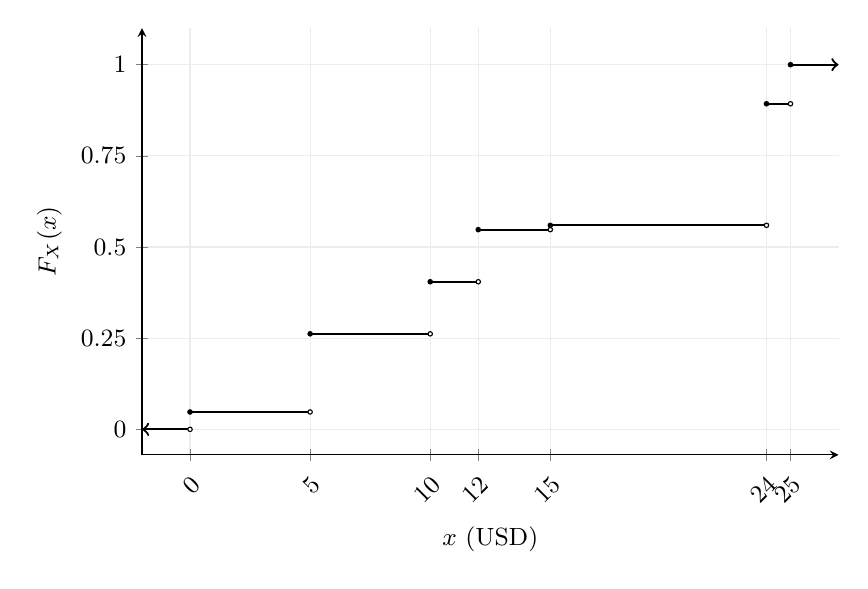
\begin{tikzpicture}
\begin{axis}[keyaxis,width=.86\linewidth,height=7cm,xmin=-2,xmax=27,ymin=-.07,ymax=1.1,xtick={0,5,10,12,15,24,25},xticklabel style={rotate=45,anchor=north east},ytick={0,.25,.5,.75,1},ylabel={$F_X(x)$}]

\addplot[thick,<-] coordinates {(-2,0)(0,0)};

\addplot[thick] coordinates {(0,4/84)(5,4/84)};

\addplot[thick] coordinates {(5,22/84)(10,22/84)};

\addplot[thick] coordinates {(10,34/84)(12,34/84)};

\addplot[thick] coordinates {(12,46/84)(15,46/84)};

\addplot[thick] coordinates {(15,47/84)(24,47/84)};

\addplot[thick] coordinates {(24,75/84)(25,75/84)};

\addplot[thick,->] coordinates {(25,1)(27,1)};

\addplot[only marks,mark=*,mark size=.8pt,mark options={fill=white}] coordinates {(0,0/84)(5,4/84)(10,22/84)(12,34/84)(15,46/84)(24,47/84)(25,75/84)};

\addplot[only marks,mark=*,mark size=.8pt] coordinates {(0,4/84)(5,22/84)(10,34/84)(12,46/84)(15,47/84)(24,75/84)(25,84/84)};

\end{axis}\end{tikzpicture}\end{center}

\textbf{CDF checks.} The table covers every real cutoff. Heights lie in $[0,1]$ and never decrease. Each horizontal segment includes its left endpoint and excludes its right endpoint: the filled point gives the value at a jump, so the CDF is right-continuous. Arrows extend the tails to $-\infty$ and $+\infty$, where the limits are 0 and 1.

In support order, subtracting successive cumulative numerators (starting at zero) gives $4,18,12,12,1,28,9$. Hence each jump is its PMF mass over $84$: $F_X(a)-F_X(a^-)=p_X(a)$. At unsupported cutoffs both the jump and the mass are zero.

\textbf{Proposed partial credit.} 0.75 for cumulative sums; 0.75 for the complete interval table and tails; 0.75 for the labeled, correctly spaced step graph and endpoints; 0.75 for the CDF and jump checks. Total: 3 points.

\par\vspace{3mm}\secInicio[][sec:q6]

\textbf{Scoring reconciliation.} Question 6 gives $3+3=6$ points for C2. C2 gives $2+2+4+6=14$ points; its independent passing threshold is 4 points. C1 gives $3+3=6$ points; its independent passing threshold is also 4 points. The overall available total is $6+14=20$ points, with no transfer between criteria.

\end{document}
